\documentclass[10pt,a4paper]{article}
\usepackage[UTF8,fontset = windows]{ctex}
\setCJKmainfont[BoldFont=黑体,ItalicFont=楷体]{华文中宋}
\usepackage{amssymb,amsmath,amsfonts,amsthm,mathrsfs,dsfont,graphicx}
\usepackage{ifthen,indentfirst,enumerate,color,titletoc}
\usepackage{tikz}
\usepackage{multicol}
\usepackage{makecell}
\usepackage{longtable}
\usetikzlibrary{arrows,calc,intersections,patterns,decorations.pathreplacing,3d,angles,quotes,positioning}
\usepackage[bf,small,indentafter,pagestyles]{titlesec}
\usepackage[top=1in, bottom=1in,left=0.8in,right=0.8in]{geometry}
\renewcommand{\baselinestretch}{1.65}
\newtheorem{defi}{定义~}
\newtheorem{eg}{例~}
\newtheorem{ex}{~}
\newtheorem{rem}{注~}
\newtheorem{thm}{定理~}
\newtheorem{coro}{推论~}
\newtheorem{axiom}{公理~}
\newtheorem{prop}{性质~}
\newcommand{\blank}[1]{\underline{\hbox to #1pt{}}}
\newcommand{\bracket}[1]{(\hbox to #1pt{})}
\newcommand{\onech}[4]{\par\begin{tabular}{p{.9\textwidth}}
A.~#1\\
B.~#2\\
C.~#3\\
D.~#4
\end{tabular}}
\newcommand{\twoch}[4]{\par\begin{tabular}{p{.46\textwidth}p{.46\textwidth}}
A.~#1& B.~#2\\
C.~#3& D.~#4
\end{tabular}}
\newcommand{\vartwoch}[4]{\par\begin{tabular}{p{.46\textwidth}p{.46\textwidth}}
(1)~#1& (2)~#2\\
(3)~#3& (4)~#4
\end{tabular}}
\newcommand{\fourch}[4]{\par\begin{tabular}{p{.23\textwidth}p{.23\textwidth}p{.23\textwidth}p{.23\textwidth}}
A.~#1 &B.~#2& C.~#3& D.~#4
\end{tabular}}
\newcommand{\varfourch}[4]{\par\begin{tabular}{p{.23\textwidth}p{.23\textwidth}p{.23\textwidth}p{.23\textwidth}}
(1)~#1 &(2)~#2& (3)~#3& (4)~#4
\end{tabular}}
\begin{document}

\begin{enumerate}[1.]

\item {\tiny (000076)}求函数$y=\dfrac1{2-x}+\sqrt{x^2-1}$的定义域.
\item {\tiny (000567)}函数$f(x)=\sqrt{1-\lg x}$的定义域为\blank{50}.
\item {\tiny (000607)}函数$y=\log_2(1-\dfrac1x)$的定义域为\blank{50}.
\item {\tiny (000646)}函数$y=\sqrt{2x-x^2}$的定义域是\blank{50}.
\item {\tiny (000778)}函数$y=\sqrt{\lg(x+2)}$的定义域为\blank{50}.
\item {\tiny (000845)}已知函数$f(x)=\lg (\sqrt{x^2+1}+ax)$的定义域为$\mathbf{R}$, 则实数$a$的取值范围是\blank{50}.
\item {\tiny (000868)}函数$f(x)=\dfrac{\sqrt{x+2}}{x-1}$的定义域为\blank{50}.
\item {\tiny (000931)}函数$y=\log_3 (x-1)$的定义域是\blank{50}.
\item {\tiny (001164)}写出下列函数的定义域(写在对应关系的右边):\\ 
(1) $f(x)=\dfrac{6}{x^2-3x+2}$;\\ 
(2) $f(x)=\dfrac{3x-1}{2x^3+4x^2+x-7}$;\\ 
(3) $f(x)=\dfrac{\sqrt[3]{4x+8}}{\sqrt{3x-2}}$;\\ 
(4) $f(x)=\sqrt{2x-1}+\sqrt{1-2x}+4$;\\ 
(5) $f(x)=\sqrt{x^2-4}$;\\ 
(6) $f(x)=\dfrac{\sqrt{2x+1}}{x-3}$.
\item {\tiny (001262)}已知函数$y=f(2x-1)$的定义域为$[0,3]$, 则函数$y=f(3x+1)$的定义域为\blank{50}.
\item {\tiny (001274)}已知$k$是实数, 函数$y=\sqrt{kx^2+2(k+2)x+3(4k-1)}$的定义域为$\mathbf{R}$, 则$k$的取值范围为\blank{50}.
\item {\tiny (002820)}若实数$x$、$y$、$m$满足$|x-m|>|y-m|$, 则称$x$比$y$远离$m$.\\
(1) 若$x^2-1$比$1$远离$0$, 求$x$的取值范围;\\
(2)定义: 在$\mathbf{R}$上的函数$f(x)$等于$x^2$和$x+2$中远离$0$的那个值. 求证: $f(x)\ge 1$在$\mathbf{R}$上恒成立.
\item {\tiny (002831)}已知函数$f(x)=\sqrt{ax^2+x+1}$.\\
(1) 若函数$y=f(x)$的定义域为$(-\infty ,+\infty)$, 求实数$a$的取值范围;\\
(2) 若函数$y=f(x)$的值域为$[0,+\infty)$, 求实数$a$的取值范围.
\item {\tiny (002833)}已知函数$y=f(x)$的定义域为$[1,4]$, 则函数$y=\dfrac{f(2x)}{x-2}$的定义域是\blank{50}.
\item {\tiny (002968)}*已知函数$f(x)=2+\log_3 x\ (3\le x\le 27)$.\\
(1) 求函数$y=f(x^2)$的定义域;\\
(2) 求函数$g(x)={[f(x)]}^2+f(x^2)$的值域.
\item {\tiny (009508)}下列四组函数中, 同组的两个函数是相同函数的是\bracket{20}.
\twoch{$y=|x|$与$y=(\sqrt x)^2$}{$y=x$与$y=\mathrm{e}^{\ln x}$}{$y=x$与$y=\sqrt[5]{x^5}$}{$y=x$与$y=(\dfrac 1x)^{-1}$}
\item {\tiny (005300)}在\textcircled{1} $y=x$与$y=\sqrt {x^2}$; \textcircled{2} $y=\sqrt {x^2}$与$y=(\sqrt x)^2$; \textcircled{3} $y=|x|$与$y=\dfrac{x^2}x$; \textcircled{4} $y=|x|$与$y=\sqrt {x^2}$; \textcircled{5} $y=x^0$与$y=1$这五组函数中, 表示同一函数的组数是\bracket{20}.
\fourch{$0$}{$1$}{$2$}{$3$}
\item {\tiny (000342)}若函数$f(x)=\begin{cases}    2^x, & x\le 0, \\ -x^2+m, & x>0 \end{cases}$的值域为$(-\infty ,1]$, 则实数$m$的取值范围是\blank{50}.
\item {\tiny (001165)}(1) 函数$f(x)=x^2, \ x \in [0,1]$的值域为\blank{50};\\ 
(2) 函数$f(x)=-x, \ x \in [-1,0)$的值域为\blank{50};\\ 
(3) 函数$f(x)=\left\{\begin{array}{cc}x^2,&0\le x\le 1,\\-x,&-1\le x<0.\end{array}\right.$的值域为\blank{50}.
\item {\tiny (001238)}函数$y=x^2-3x+1, \ x \in [1,4]$的值域为\blank{80}.
\item {\tiny (001239)}函数$y=\dfrac{2x+3}{x-1}$的值域为\blank{80}.
\item {\tiny (001242)}函数$y=\sqrt{1+x}+2x$的值域为\blank{80}.
\item {\tiny (001243)}函数$y=|x-3|-|x-10|$的值域为\blank{80}.
\item {\tiny (001244)}函数$y=|x-3|+|x-10|+|x+1|+|x+2|$的值域为\blank{80}.
\item {\tiny (001245)}函数$y=||x-3|+x|$的值域为\blank{80}.
\item {\tiny (001250)}函数$y=\sqrt{1+\sqrt{1+\sqrt{1+\sqrt{x^2+64}}}}$的值域为\blank{80}.
\item {\tiny (001252)}函数$y=\dfrac{1}{x^2+x+1}$的值域为\blank{80}.
\item {\tiny (001266)}写出下列函数的值域.\\ 
(1) $y=3x+1, \ x \in [-2,5]$; \blank{80}\\ 
(2) $y=|2x+1|, \ x \in [-1,3]$; \blank{80}\\ 
(3) $y=\dfrac{x-1}{2x+3}$; \blank{80}\\ 
(4) $y=\dfrac{|x|+1}{|x|-1}$; \blank{80}\\ 
(5) $y=\dfrac{|x+3|}{x-4}, \ x \in [-4,0]$; \blank{80}\\ 
(6) $y=\dfrac{2x+1}{|x+1|-|x|}$; \blank{80}
\item {\tiny (001275)}已知$k$是实数, 函数$y=\sqrt{kx^2+2(k+2)x+3(4k-1)}$的值域为$[0,+\infty)$, 则$k$的取值范围为\blank{50}.
\item {\tiny (002987)}函数$f(x)=ax^2+bx+c$ 与函数$g(x)=cx^2+bx+a$($ac\ne 0,\ a\ne c)$的值域分别为$M$、$N$, 则下列结论正确的是\blank{50}.
\fourch{$M=N$}{$M\subseteq N$}{$M\supseteq N$}{$M\cap N\ne \varnothing$}
\item {\tiny (002994)}函数$y=\log_{\frac 12}(-x^2+2x+3)$的值域是\blank{50}.
\item {\tiny (003862)}如图, 直角梯形$OABC$中, $AB\parallel OC$, $AB=1$, $OC=BC=2$, 直线$l: x=t$截此梯形所得位于$l$左方图形面积为$S$, 
\begin{center}
	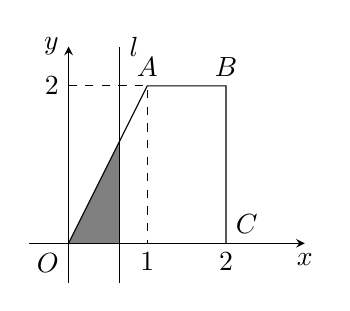
\begin{tikzpicture}[samples=200,>=stealth]
	\fill [gray] (0,0)--(0.65,0)--(0.65,1.3)--cycle;
	\draw [->] (-0.5,0)--(0,0) node [below left] {$O$} --(3,0) node [below] {$x$};
	\draw [->] (0,-0.5)--(0,2.5) node [left] {$y$};
	\draw (0,0)--(1,2) node [above] {$A$}--(2,2) node [above] {$B$}--(2,0) node [above right] {$C$};
	\draw (0.65,-0.5)--(0.65,2.5) node [right] {$l$};
	\draw [dashed] (0,2) node [left] {$2$} --(1,2)--(1,0) node [below] {$1$};
	\draw (2,0) node [below] {$2$};
	
	\end{tikzpicture}
\end{center}
则函数$S=f(t)$的图像大致为\blank{30}.
\fourch{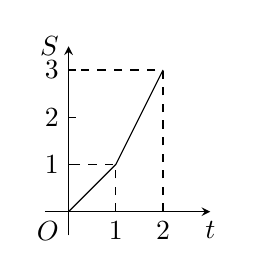
\begin{tikzpicture}[>=stealth]
	\draw [->] (-0.3,0)--(0,0) node [below left] {$O$} --(1.8,0) node [below] {$t$};
	\draw [->] (0,-0.3)--(0,2.1) node [left] {$S$};
	\draw (0.6,0) node [below] {$1$}--(0.6,0.1);
	\draw (1.2,0) node [below] {$2$}--(1.2,0.1);
	\draw (0,0.6) node [left] {$1$}--(0.1,0.6);
	\draw (0,1.2) node [left] {$2$}--(0.1,1.2);
	\draw (0,1.8) node [left] {$3$}--(0.1,1.8);
	\draw (0,0)--(0.6,0.6)--(1.2,1.8);
	\draw [dashed] (0.6,0)--(0.6,0.6)--(0,0.6);
	\draw [dashed] (1.2,0)--(1.2,1.8)--(0,1.8);
	\end{tikzpicture}}{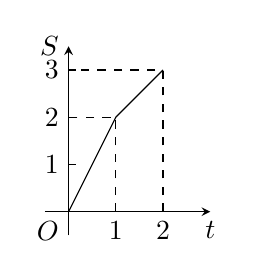
\begin{tikzpicture}[>=stealth]
	\draw [->] (-0.3,0)--(0,0) node [below left] {$O$} --(1.8,0) node [below] {$t$};
	\draw [->] (0,-0.3)--(0,2.1) node [left] {$S$};
	\draw (0.6,0) node [below] {$1$}--(0.6,0.1);
	\draw (1.2,0) node [below] {$2$}--(1.2,0.1);
	\draw (0,0.6) node [left] {$1$}--(0.1,0.6);
	\draw (0,1.2) node [left] {$2$}--(0.1,1.2);
	\draw (0,1.8) node [left] {$3$}--(0.1,1.8);
	\draw (0,0)--(0.6,1.2)--(1.2,1.8);
	\draw [dashed] (0.6,0)--(0.6,1.2)--(0,1.2);
	\draw [dashed] (1.2,0)--(1.2,1.8)--(0,1.8);
	\end{tikzpicture}}{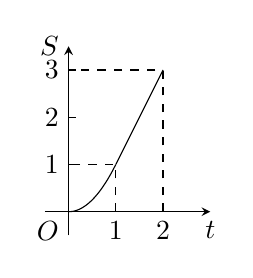
\begin{tikzpicture}[>=stealth,samples=200]
	\draw [->] (-0.3,0)--(0,0) node [below left] {$O$} --(1.8,0) node [below] {$t$};
	\draw [->] (0,-0.3)--(0,2.1) node [left] {$S$};
	\draw (0.6,0) node [below] {$1$}--(0.6,0.1);
	\draw (1.2,0) node [below] {$2$}--(1.2,0.1);
	\draw (0,0.6) node [left] {$1$}--(0.1,0.6);
	\draw (0,1.2) node [left] {$2$}--(0.1,1.2);
	\draw (0,1.8) node [left] {$3$}--(0.1,1.8);
	\draw [domain=0:1] plot ({\x*0.6},{\x*\x*0.6});
	\draw (0.6,0.6)--(1.2,1.8);
	\draw [dashed] (0.6,0)--(0.6,0.6)--(0,0.6);
	\draw [dashed] (1.2,0)--(1.2,1.8)--(0,1.8);
	\end{tikzpicture}}{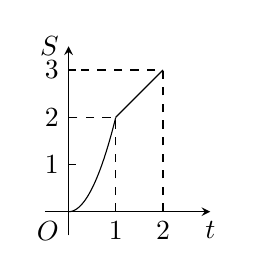
\begin{tikzpicture}[>=stealth,samples=200]
	\draw [->] (-0.3,0)--(0,0) node [below left] {$O$} --(1.8,0) node [below] {$t$};
	\draw [->] (0,-0.3)--(0,2.1) node [left] {$S$};
	\draw (0.6,0) node [below] {$1$}--(0.6,0.1);
	\draw (1.2,0) node [below] {$2$}--(1.2,0.1);
	\draw (0,0.6) node [left] {$1$}--(0.1,0.6);
	\draw (0,1.2) node [left] {$2$}--(0.1,1.2);
	\draw (0,1.8) node [left] {$3$}--(0.1,1.8);
	\draw [domain=0:1] plot ({\x*0.6},{2*\x*\x*0.6});
	\draw (0.6,1.2)--(1.2,1.8);
	\draw [dashed] (0.6,0)--(0.6,1.2)--(0,1.2);
	\draw [dashed] (1.2,0)--(1.2,1.8)--(0,1.8);
	\end{tikzpicture}}
\item {\tiny (001176)}求证: 函数$y=x^3$的图像不是一条直线(本题不能使用斜率的概念).
\item {\tiny (003884)}已知函数$y=f(x)$的定义域为$\{x|-3\le x\le 8, \ x\ne 5\}$, 值域为$\{y|-1\le y\le 2, \ y\ne 0\}$. 下列关于函数$y=f(x)$的说法: \textcircled{1} 当$x=-3$时, $y=-1$; \textcircled{2} 将$y=f(x)$的图像补上$(5,0)$, 得到的图像必定是一条连续的曲线; \textcircled{3} $y=f(x)$是$[-3,5)$上的单调函数; \textcircled{4} $y=f(x)$的图像与坐标轴只有一个交点. 其中正确的命题是\blank{50}.
\item {\tiny (005303)}函数$y=x+\dfrac{|x|}x$的图像是\bracket{20}.
\fourch{\begin{tikzpicture}[scale = 0.7,>=latex]
\draw [->] (-2,0) -- (2,0) node [below] {$x$};
\draw [->] (0,-2) -- (0,2) node [left] {$y$};
\draw (0,0) node [below right] {$O$};
\draw (-1,0) node [below] {$-1$} (0,1) node [right] {$1$};
\draw (-2,-1) -- (1,2);
\filldraw [white] (0,1) circle (0.05);
\draw (0,1) circle (0.05);
\end{tikzpicture}}{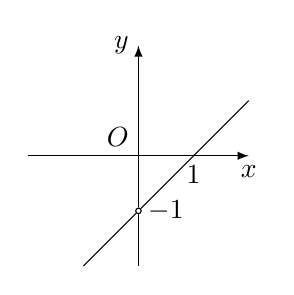
\begin{tikzpicture}[scale = 0.7,>=latex]
\draw [->] (-2,0) -- (2,0) node [below] {$x$};
\draw [->] (0,-2) -- (0,2) node [left] {$y$};
\draw (0,0) node [above left] {$O$};
\draw (1,0) node [below] {$1$} (0,-1) node [right] {$-1$};
\draw (-1,-2) -- (2,1);
\filldraw [white] (0,-1) circle (0.05);
\draw (0,-1) circle (0.05);
\end{tikzpicture}}{\begin{tikzpicture}[scale = 0.7,>=latex]
\draw [->] (-2,0) -- (2,0) node [below] {$x$};
\draw [->] (0,-2) -- (0,2) node [left] {$y$};
\draw (0,0) node [below right] {$O$};
\draw (1,0.1) -- (1,0) node [below] {$1$} (0,-1) node [right] {$-1$} (0,1) node [right] {$1$} (-1,0.1) -- (-1,0) node [below] {$-1$};
\draw (-1,-2) -- (0,-1) (0,1) -- (1,2);
\filldraw [white] (0,-1) circle (0.05);
\draw (0,-1) circle (0.05);
\filldraw [white] (0,1) circle (0.05);
\draw (0,1) circle (0.05);
\end{tikzpicture}}{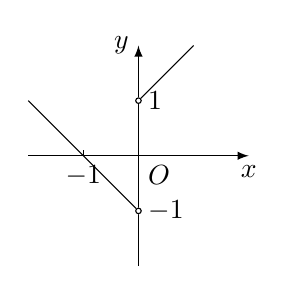
\begin{tikzpicture}[scale = 0.7,>=latex]
\draw [->] (-2,0) -- (2,0) node [below] {$x$};
\draw [->] (0,-2) -- (0,2) node [left] {$y$};
\draw (0,0) node [below right] {$O$};
\draw (0,-1) node [right] {$-1$} (0,1) node [right] {$1$} (-1,0.1) -- (-1,0) node [below] {$-1$};
\draw (-2,1) -- (0,-1) (0,1) -- (1,2);
\filldraw [white] (0,-1) circle (0.05);
\draw (0,-1) circle (0.05);
\filldraw [white] (0,1) circle (0.05);
\draw (0,1) circle (0.05);
\end{tikzpicture}}
\item {\tiny (007942)}打开水龙头, 让水匀速地注入一个杯子内, 随着时间的增加, 杯中水面的高度不断增加, 直至水满溢出.在这个过程中, 杯中水面的高度$h$关于注水时间$t$的函数为$h=f(t)$.
\begin{center}
    \begin{tikzpicture}[scale = 0.6]
        \draw (-2,3) arc (180:-180:2 and 0.5);
        \draw (-1.95,3) arc (180:-180:1.95 and 0.475);
        \draw (-2,3) -- (-2,0) (2,3) -- (2,0);
        \draw (-2,0) arc (180:360:2 and 0.5);
        \draw [dashed] (-2,0) arc (180:0:2 and 0.5);
        \draw [dashed] (0,0) ellipse (0.6 and 0.15) (-0.6,0) arc (90:0:0.4) (0.6,0) arc (90:180:0.4);
        \draw [dashed] (-0.2,-0.4) -- (-0.2,-0.6) (0.2,-0.4) -- (0.2,-0.6);
        \draw (-0.2,-0.5) -- (-0.2, -1.6) (0.2,-0.5) -- (0.2,-1.6) 
        (-0.6,-2) arc (270:360:0.4) (0.6,-2) arc (270:180:0.4);
        \draw (-1,-2) arc (180:-180:1 and 0.25);
        \draw (-1,-2.05) arc (180:360:1 and 0.25);
        \draw (0,-2.5) node [below] {甲};
    \end{tikzpicture}
    \begin{tikzpicture}[scale = 0.6]
        \draw (-2,3) arc (180:-180:2 and 0.5);
        \draw (-1.95,3) arc (180:-180:1.95 and 0.475);
        \draw (-2,3) -- (-0.2,0) (2,3) -- (0.2,0);
        \draw (-0.2,0) arc (180:360:0.2 and 0.05);
        \draw [dashed] (-0.2,0) arc (180:0:0.2 and 0.05);
        \draw (-0.2,0) -- (-0.2, -1.6) (0.2,0) -- (0.2,-1.6) 
        (-0.6,-2) arc (270:360:0.4) (0.6,-2) arc (270:180:0.4);
        \draw (-1,-2) arc (180:-180:1 and 0.25);
        \draw (-1,-2.05) arc (180:360:1 and 0.25);
        \draw (0,-2.5) node [below] {乙};
    \end{tikzpicture}
\end{center}
(1) 如果甲杯、乙杯的形状分别如图所示, 那么下列草图中, 甲杯相应函数$h=f(t)$的图像是\blank{50}, 乙杯相应函数$h=f(t)$的图像是\blank{50}.(只有杯子的圆柱和圆锥形部分可以盛水)
\begin{center}
    \begin{tikzpicture}[>=latex]
        \draw [->] (-0.5,0) -- (2.5,0) node [below] {$t$};
        \draw [->] (0,-0.5) -- (0,2.5) node [left] {$h$};
        \draw (0,0) node [below left] {$O$};
        \draw (0,0) -- (2,2);
        \draw (1,-0.5) node [below] {(a)};
    \end{tikzpicture}
    \begin{tikzpicture}[>=latex]
        \draw [->] (-0.5,0) -- (2.5,0) node [below] {$t$};
        \draw [->] (0,-0.5) -- (0,2.5) node [left] {$h$};
        \draw (0,0) node [below left] {$O$};
        \draw (0,0) -- (1.5,1.5) -- (2,1.5);
        \draw (1,-0.5) node [below] {(b)};
    \end{tikzpicture}
    \begin{tikzpicture}[>=latex]
        \draw [->] (-0.5,0) -- (2.5,0) node [below] {$t$};
        \draw [->] (0,-0.5) -- (0,2.5) node [left] {$h$};
        \draw (0,0) node [below left] {$O$};
        \draw (0,0) arc (180:90:0.5 and 1.5) -- (2,1.5);
        \draw (1,-0.5) node [below] {(c)};
    \end{tikzpicture}
    \begin{tikzpicture}[>=latex]
        \draw [->] (-0.5,0) -- (2.5,0) node [below] {$t$};
        \draw [->] (0,-0.5) -- (0,2.5) node [left] {$h$};
        \draw (0,0) node [below left] {$O$};
        \draw (0,0) arc (270:360:0.5 and 1.5) -- (2,1.5);
        \draw (1,-0.5) node [below] {(d)};
    \end{tikzpicture}
\end{center}
(2) 下列是两个杯子相应函数$h=f(t)$的图像, 试说明这两个杯子形状有何差别.
\begin{center}
    \begin{tikzpicture}[>=latex]
        \draw [->] (-0.5,0) -- (2.5,0) node [below] {$t$};
        \draw [->] (0,-0.5) -- (0,2.5) node [left] {$h$};
        \draw (0,0) node [below left] {$O$};
        \draw (0,0) -- (0.5,1.5) -- (2,1.5);
        \draw (1,-0.5) node [below] {(e)};
    \end{tikzpicture}
    \begin{tikzpicture}[>=latex]
        \draw [->] (-0.5,0) -- (2.5,0) node [below] {$t$};
        \draw [->] (0,-0.5) -- (0,2.5) node [left] {$h$};
        \draw (0,0) node [below left] {$O$};
        \draw (0,0) -- (1.5,1.5) -- (2,1.5);
        \draw (1,-0.5) node [below] {(f)};
    \end{tikzpicture}
\end{center}
\item {\tiny (003936)}函数$y=\ln(\cos x) \ \left(-\dfrac{\pi}{2}<x<\dfrac{\pi}{2}\right)$的大致图像是\blank{30}.
\fourch{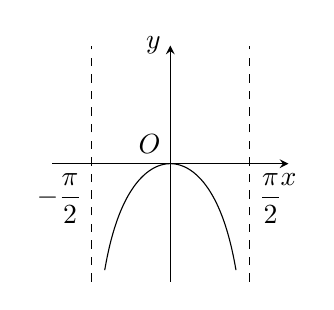
\begin{tikzpicture}[samples=200,>=stealth]
	\draw [->](-1.5,0)--(0,0) node [above left] {$O$}--(1.5,0) node [below] {$x$};
	\draw [->](0,-1.5)--(0,1.5) node [left] {$y$};
	\draw [dashed] (-1,-1.5)--(-1,1.5) (1,-1.5)--(1,1.5);
	\draw (-1,0) node [below left] {$-\dfrac{\pi}{2}$};
	\draw (1,0) node  [below right] {$\dfrac{\pi}{2}$};
	\draw [domain=-75:75] plot ({\x/90},{ln(cos(\x))});
	\end{tikzpicture}}{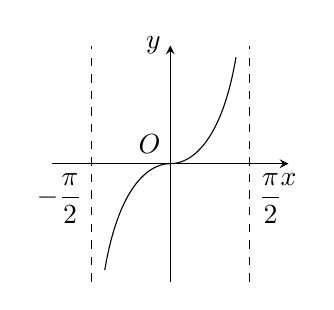
\begin{tikzpicture}[samples=200,>=stealth]
	\draw [->](-1.5,0)--(0,0) node [above left] {$O$}--(1.5,0) node [below] {$x$};
	\draw [->](0,-1.5)--(0,1.5) node [left] {$y$};
	\draw [dashed] (-1,-1.5)--(-1,1.5) (1,-1.5)--(1,1.5);
	\draw (-1,0) node [below left] {$-\dfrac{\pi}{2}$};
	\draw (1,0) node  [below right] {$\dfrac{\pi}{2}$};
	\draw [domain=-75:0] plot ({\x/90},{ln(cos(\x))});
	\draw [domain=0:75] plot ({\x/90},{-ln(cos(\x))});
	\end{tikzpicture}}{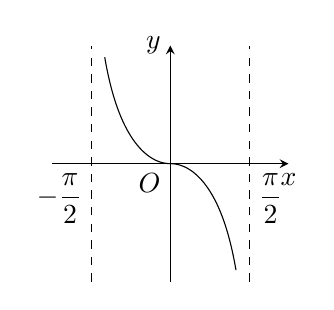
\begin{tikzpicture}[samples=200,>=stealth]
	\draw [->](-1.5,0)--(0,0) node [below left] {$O$}--(1.5,0) node [below] {$x$};
	\draw [->](0,-1.5)--(0,1.5) node [left] {$y$};
	\draw [dashed] (-1,-1.5)--(-1,1.5) (1,-1.5)--(1,1.5);
	\draw (-1,0) node [below left] {$-\dfrac{\pi}{2}$};
	\draw (1,0) node  [below right] {$\dfrac{\pi}{2}$};
	\draw [domain=-75:0] plot ({\x/90},{-ln(cos(\x))});
	\draw [domain=0:75] plot ({\x/90},{ln(cos(\x))});
	\end{tikzpicture}}{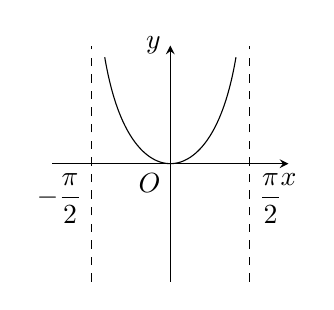
\begin{tikzpicture}[samples=200,>=stealth]
	\draw [->](-1.5,0)--(0,0) node [below left] {$O$}--(1.5,0) node [below] {$x$};
	\draw [->](0,-1.5)--(0,1.5) node [left] {$y$};
	\draw [dashed] (-1,-1.5)--(-1,1.5) (1,-1.5)--(1,1.5);
	\draw (-1,0) node [below left] {$-\dfrac{\pi}{2}$};
	\draw (1,0) node  [below right] {$\dfrac{\pi}{2}$};
	\draw [domain=-75:75] plot ({\x/90},{-ln(cos(\x))});
	\end{tikzpicture}}
\item {\tiny (002838)}*设$D$是含数$1$的有限实数集, $f(x)$是定义在$D$上的函数, 若$f(x)$的图像绕原点逆时针旋转$\dfrac \pi6$后与原图像重合, 则在以下各项中, $f(1)$的可能取值只能是\bracket{20}
\fourch{$\sqrt3$}{$\dfrac{\sqrt{3}}2$}{$\dfrac{\sqrt{3}}3$}{$0$}
\item {\tiny (007984)}下列图形中, 能作为某个函数的图像的只能是\bracket{20}.
\fourch{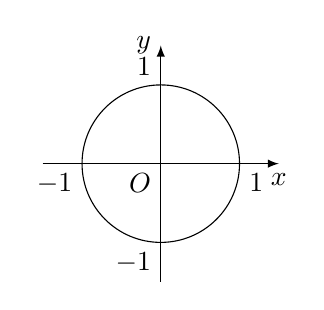
\begin{tikzpicture}[>=latex]
    \draw [->] (-1.5,0) -- (1.5,0) node [below] {$x$};
    \draw [->] (0,-1.5) -- (0,1.5) node [left] {$y$};
    \draw (0,0) node [below left] {$O$};
    \draw (1,0) node [below right] {$1$} (-1,0) node [below left] {$-1$} (0,1) node [above left] {$1$} (0,-1) node [below left] {$-1$};
    \draw (0,0) circle (1);
\end{tikzpicture}
}{\begin{tikzpicture}[>=latex]
    \draw [->] (-1.5,0) -- (1.5,0) node [below] {$x$};
    \draw [->] (0,-1.5) -- (0,1.5) node [left] {$y$};
    \draw (0,0) node [below left] {$O$};
    \draw (1,0) node [below right] {$1$} (0,1) node [above left] {$1$} (0,-1) node [below left] {$-1$};
    \draw (0,1) arc (90:-90:1);
\end{tikzpicture}}{\begin{tikzpicture}[>=latex]
    \draw [->] (-1.5,0) -- (1.5,0) node [below] {$x$};
    \draw [->] (0,-1.5) -- (0,1.5) node [left] {$y$};
    \draw (0,0) node [below left] {$O$};
    \draw (1,0) node [below right] {$1$} (0,1) node [above left] {$1$} (0,-1) node [below left] {$-1$} (-1,0) node [below left] {$-1$};
    \draw (0,1) arc (90:0:1) (0,-1) arc (270:180:1);
    \filldraw [fill = white, draw = black] (0,1) circle (0.05) (0,-1) circle (0.05);
\end{tikzpicture}}{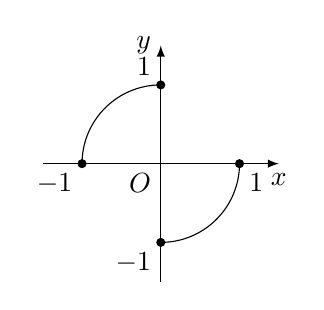
\begin{tikzpicture}[>=latex]
    \draw [->] (-1.5,0) -- (1.5,0) node [below] {$x$};
    \draw [->] (0,-1.5) -- (0,1.5) node [left] {$y$};
    \draw (0,0) node [below left] {$O$};
    \draw (1,0) node [below right] {$1$} (0,1) node [above left] {$1$} (0,-1) node [below left] {$-1$} (-1,0) node [below left] {$-1$};
    \draw (0,1) arc (90:180:1) (0,-1) arc (270:360:1);
    \filldraw (0,1) circle (0.05) (0,-1) circle (0.05) (1,0) circle (0.05) (-1,0) circle (0.05);
\end{tikzpicture}}
\item {\tiny (000083)}邮局规定: 当邮件质量不超过$100$g时, 每$20$g邮费$0.8$元, 且不足$20$g时按$20$g计算; 超过$100$g时, 超过$100$g的部分按每$100$g邮费$2$元计算, 且不足$100$g按$100$g
计算; 同时规定邮件总质量不得超过$2000$g. 请写出邮费关于邮件质量的函数表达式, 并计算$50$g和$500$g的邮件分别收多少邮费.
\item {\tiny (009511)}根据下图的函数图像, 用解析法表示$y$关于$x$的函数.
\begin{center}
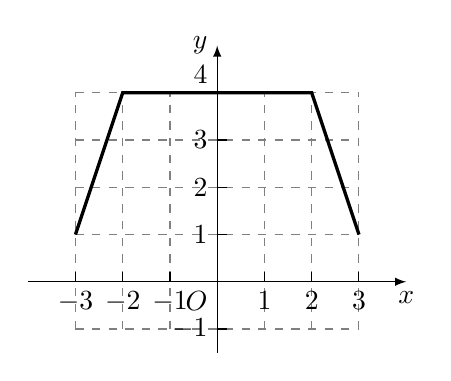
\begin{tikzpicture}[>=latex,scale = 0.6]
\foreach \i in {-3,-2,...,3}
{\draw [dashed, gray] (\i,-1) -- (\i,4);};
\foreach \i in {-1,0,...,4}
{\draw [dashed, gray] (-3,\i) -- (3,\i);};
\draw [->] (-4,0) -- (4,0) node [below] {$x$};
\draw [->] (0,-1.5) -- (0,5) node [left] {$y$};
\draw (0,0) node [below left] {$O$};
\draw [very thick] (-3,1) -- (-2,4) -- (2,4) -- (3,1);
\foreach \i in {-3,-2,-1,1,2,3}
{\draw (\i,0.2) -- (\i,0) node [below] {$\i$};};
\foreach \i in {-1,1,2,3}
{\draw (0.2,\i) -- (0,\i) node [left] {$\i$};};
\draw (0,4) node [above left] {$4$};
\end{tikzpicture}
\end{center}
\item {\tiny (011383)}在某种计算机语言中, 有一种函数$y=\texttt{INT}(x)$叫做取整函数(也叫高斯函数), 它表示$y$等于不超过$x$的最大整数, 如$\texttt{INT}(0.9)=0$, $\texttt{INT}(3.14)=3$. 已知$a_n=\texttt{INT}(\dfrac 27\times 10^n)$, $b_1=a_1$, $b_n=a_n-10a_{n-1}$($n\in \mathbf{N}^*$且$n\ge 2$), 则$b_{2018}$等于\bracket{20}.
\fourch{$2$}{$5$}{$7$}{$8$}
\item {\tiny (011126)}符号$[x]$表示不超过$x$的最大整数, 如$[\pi]=3$, $[-1.08]=-2$, 定义函数$\{x\}=x-[x]$, 那么下列命题中正确的序号是\bracket{20}.\\
\textcircled{1} 函数$\{x\}$的定义域为$\mathbf{R}$, 值域为$[0,1]$; \textcircled{2} 方程$\{x\}=\dfrac 12$有无数解; \textcircled{3} 函数$\{x\}$是周期函数; \textcircled{4} 函数$\{x\}$是增函数.
\fourch{\textcircled{1}\textcircled{2}}{\textcircled{3}\textcircled{3}}{\textcircled{3}\textcircled{4}}{\textcircled{4}\textcircled{1}}
\item {\tiny (002863)}函数$y=\dfrac 1{x^2-4x+5}$的图像关于\bracket{20}.
\fourch{$y$轴对称}{原点对称}{直线$x=2$对称}{点$(2,1)$对称}
\item {\tiny (007949)}已知幂函数$f(x)$的定义域是$(+\infty ,0)\cup (0,+\infty)$, 且它的图像关于$y$轴对称, 写出一个满足要求的幂函数$f(x)$.
\item {\tiny (005508)}$f(x)+f(2-x)+2=0$对任何实数$x$都成立, 则$f(x)$的图像\bracket{20}.
\twoch{关于直线$x=1$成轴对称图形}{关于直线$x=2$成轴对称图形}{关于点$(1, -1)$成中心对称图形}{关于点$(-1,1)$成中心对称图形}
\item {\tiny (002879)}已知定义域为$\mathbf{R}$的函数$y=f(x)$是偶函数, 并且其图像关于直线$x=1$对称.\\
(1) 若$f(0)=1$, $f(1)=2$, 求$f(15)+2f(20)$的值;\\
(2) 设$x\in [0,1]$时, $f(x)=x^3$.\\
\textcircled{1} $1<x\le 2$时, 求$y=f(x)$的解析式;\\
\textcircled{2} $-2\le x<0$时, 求$y=f(x)$的解析式;\\
\textcircled{3} 求函数$y=f(x)-\dfrac 18$在$[-2,2]$上的所有零点;\\
\textcircled{4} 求$y=f(x)$在$\mathbf{R}$上的解析式.
\item {\tiny (000734)}给出下列函数: \textcircled{1} $y=x+\dfrac1x$; \textcircled{2} $y={x^2}+x$; \textcircled{3} $y={2^{|x|}}$; \textcircled{4} $y={x^{\dfrac23}}$; \textcircled{5} $y=\tan x$; \textcircled{6} $y=\sin(\arccos x)$; \textcircled{7} $y=\lg(x+\sqrt{{x^2}+4})-\lg 2$. 从这$7$个函数中任取两个函数, 则其中一个是奇函数另一个是偶函数的概率是\blank{50}.
\item {\tiny (001221)}判断下列函数的奇偶性, 并说明理由.\\ 
(1) $f(x)=|1+x|+|1-x|$;\\ 
(2) $f(x)=(1-x)\sqrt{\dfrac{1+x}{1-x}}$;\\ 
(3) $f(x)=\dfrac{\sqrt{x^2+1}+x-1}{\sqrt{x^2+1}+x+1}$;
\item {\tiny (002842)}给定六个函数: \textcircled{1} $y=\dfrac 1x$; \textcircled{2} $y=x^2+1$; \textcircled{3} $y={x^{-\frac 13}}$; \textcircled{4} $y=2^x$; \textcircled{5} $y=\log_2x$; \textcircled{6} $y=\sqrt{x^2-1}+\sqrt{1-x^2}$.\\
在这六个函数中, 是奇函数但不是偶函数的是\blank{50}, 是偶函数但不是奇函数的是\blank{50}, 既不是奇函数也不是偶函数的是\blank{50}, 既是奇函数又是偶函数的是\blank{50}.
\item {\tiny (002856)}判断下列函数$y=f(x)$的奇偶性, 并说明理由:\\
(1) $f(x)=x^3-\dfrac 1x$;\\
(2) $f(x)=\dfrac{|x+3|-3}{\sqrt{4-x^2}}$.
\item {\tiny (000474)}已知函数$y=f(x)$是奇函数, 当$x<0$时, $f(x)=2^x-ax$, 且$f(2)=2$, 则$a=$\blank{50}.
\item {\tiny (000863)}设定义在$\mathbf{R}$上的奇函数$y=f(x)$, 当$x>0$时, $f(x)=2^x-4$, 则不等式$f(x)\le 0$的解集是\blank{50}.
\item {\tiny (002843)}设常数$a$、$b\in \mathbf{R}$. 若定义在$[a-2,2a]$上的$f(x)=ax^2+bx$是偶函数, 则$a=$\blank{50}, $b=$\blank{50}.
\item {\tiny (002847)}设$y=f(x)$是定义在$\mathbf{R}$上的函数, 当$x\ge 0$时, $f(x)=x^2-2x$.\\
(1) 当$y=f(x)$为奇函数时, 则当$x<0$时, $f(x)$=\blank{50};\\
(2) 当$y=f(x)$为偶函数时, 则当$x<0$时, $f(x)$=\blank{50}.
\item {\tiny (002848)}设奇函数$y=f(x)$的定义域为$[-5, 5]$.若当$x\in [0,5]$时, $y=f(x)$的图像如图, 则不等式$xf(x)<0$的解是\blank{50}.
\begin{center}
    \begin{tikzpicture}[>=stealth]
        \draw [->] (-1,0) -- (6,0) node [below] {$x$};
        \draw [->] (0,-2.5) -- (0,2.5) node [left] {$y$};
        \draw (2,0) node [below] {$2$};
        \draw (5,0) node [above] {$5$};
        \draw [domain = 0:2,samples = 100] plot (\x,-\x*\x+2*\x);
        \draw [domain = 2:5,samples = 100] plot (\x, \x*\x/2-4*\x+6);
        \draw [dashed] (5,0) -- (5,-1.5);
        \draw (0,0) node [below left] {$O$};
    \end{tikzpicture}
\end{center}
\item {\tiny (002849)}若定义在$\mathbf{R}$上的两个函数$y=f(x)$、$y=g(x)$均为奇函数. 设$F(x)=af(x)+bg(x)+1$.\\
(1) 若$F(-2)=10$, 则$F(2)=$\blank{50};\\
(2) 若函数$y=F(x)$在$(0,+\infty)$上存在最大值$4$, 则$y=F(x)$在$(-\infty ,0)$上的最小值为\blank{50}.
\item {\tiny (002851)}已知函数$f(x)=x^2-2a|x-1|$, $x\in \mathbf{R}$, 常数$a\in \mathbf{R}$.\\
(1) 求证: 函数$y=f(x)$不是奇函数;\\
(2) 若函数$y=f(x)$是偶函数, 求实数$f(x)=\log_3| 2x+a |$的值.
\item {\tiny (002853)}设$y=f(x)$是定义在$\mathbf{R}$上的函数, 则下列叙述正确的是\bracket{20} .
\twoch{$y=f(x)f(-x)$是奇函数}{$y=f(x)|f(-x)|$是奇函数}{$y=f(x)-f(-x)$是偶函数	}{$y=f(x)+f(-x)$是偶函数}
\item {\tiny (002859)}是否存在实数$b$, 使得函数$g(x)=\dfrac{2^x}{{4^x}-b}$是奇函数? 若存在, 求$b$的值; 若不存在, 说明理由.
\item {\tiny (002860)}常数$a\in \mathbf{R}$. 若函数$f(x)=\lg(10^x+1)+ax$是偶函数, 则$a=$\blank{50}.
\end{enumerate}



\end{document}